\clearpage
\chapter{MARCO APLICATIVO}
% \section{IMPLEMENTACIÓN de los algoritmos de factorización}
% Esta sección detalla la implementación de los algoritmos de factorización de números enteros y los diferentes algoritmos que utilizaremos en estos, sin utilizar librerías especializadas, para incluir en el marco aplicativo de la tesis.
Para el presente capitulo es necesaria la lectura de los capítulos anteriores por los conceptos que se manejan los cuales son nombrados y fueron introducidos anteriormente.
\section{ALGORITMOS DE FACTORIZACIÓN}
Esta sección detalla la implementación de los algoritmos mostrados en el capitulo 2, se implementaran en Python sin el uso de librerías especializadas.
\subsection{ALGORITMO DE EUCLIDES}
El algoritmo de Euclides, lo usamos para encontrar el Maximo Comun Divisor (gcd) de dos números
    \subsubsection{IMPLEMENTACIÓN}
\begin{lstlisting}[language=Python]
def gcd(a, b):
    while b != 0:
        a, b = b, a % b
    return a
\end{lstlisting}
    \subsubsection{EJEMPLO NÚMERICO}
    Encontrar el Máximo Común Divisor de $252$ y $105$
    \begin{align*} 
        gcd(252, 105) &=  gcd(105, 252\%105) \\ 
        &=  gcd(105, 42) \\
        gcd(105, 42) &=  gcd(42, 105\%42) \\ 
        &=  gcd(42, 21) \\
        gcd(42, 21) &=  gcd(21, 42\%21) \\ 
        &=  gcd(21, 0) \\
        gcd(42, 21) &= 21 \Rightarrow gcd(252, 105) = 21\\
    \end{align*}

    \subsubsection{EJEMPLO DE EJECUCIÓN}
    \begin{figure}[H]
        \centering
        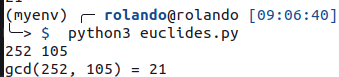
\includegraphics[width=10cm]{images/euclides_prueba.png}
        \caption{Ejecución de prueba del algoritmo de Euclides}
    \end{figure}

\subsection{ALGORITMO EXTENDIDO DE EUCLIDES}
El algoritmo extendido de Euclides, no solo encontrara los valores del Máximo Común Divisor (gcd) de dos números, sino también encontrara los valores de los coeficientes de Bézout, que son dos números tales que:
\[
    ax + by = gcd(a,b)
\]
    
    \subsubsection{IMPLEMENTACIÓN}
\begin{lstlisting}[language=Python]
def gcd_extendido(a, b):
if a == 0:
    return b, 0, 1
else:
    gcd, x1, y1 = gcd_extendido(b % a, a)
    x = y1 - (b // a) * x1
    y = x1
    return gcd, x, y
\end{lstlisting}
    
    \subsubsection{EJEMPLO NÚMERICO}
    Aplicamos el algoritmo de Euclides:
    \begin{align*} 
        252 &=  2\cdot105 + 42 \\ 
        105 &=  2\cdot42 + 21 \\
        42 &=  2\cdot21 + 0 \\ 
    \end{align*}
    
    Despejamos los residuos en los pasos del algoritmo de Euclides:

    \begin{align*} 
        42 &=  252 - 2\cdot105\\ 
        21 &=  105 - 2\cdot42\\ 
    \end{align*}

    Remplazamos 42 en la segunda ecuación:
    \begin{align*} 
        21 &=  105 - 2\cdot(252 - 2\cdot105)\\ 
        21 &=  105 - 2\cdot252 + 4\cdot105\\
        21 &=  2\cdot252 + 5\cdot105\\
        &\Rightarrow x = -2, y = 5 
    \end{align*}

    \subsubsection{EJEMPLO DE EJECUCIÓN}
    \begin{figure}[H]
        \centering
        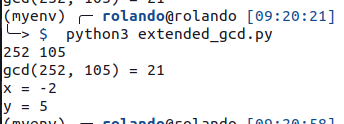
\includegraphics[width=10cm]{images/euclides_extendido_prueba.png}
        \caption{Ejecución de prueba del algoritmo extendido de Euclides}
    \end{figure}

\subsection{ALGORITMO DE EXPONENCIACIÓN MODULAR}
Con este algoritmo encontraremos de manera eficiente $f(x,a,m) = x^a \% m$
    \subsubsection{IMPLEMENTACIÓN}
\begin{lstlisting}[language=Python]
def mod_exp(base, exponente, modulo):
    resultado = 1
    base = base % modulo
    
    while exponente > 0:
        if (exponente % 2) == 1:
            resultado = (resultado * base) % modulo
        exponente = exponente >> 1
        base = (base * base) % modulo
    
    return resultado
\end{lstlisting}

    \subsubsection{EJEMPLO NÚMERICO}
    Encontrar el resultado para $25^9 \% 7$
    \begin{align*} 
        x &=  25^9 \% 7\\ 
        x &=  (25^4 \% 7)^2 (\times 25\cdot1) \% 7 \\
        x &=  ((25^2 \% 7)^2)^2 \times (25 \% 7)\\
        x &=  ((25\cdot25 \% 7)^2)^2 \times (25 \% 7)\\
        x &=  (((625 \% 7)^2)^2 \times 4)\%7\\
        x &=  (((2)^2)^2 \% 7 \times 4) mod 7\\
        x &= ((4^2)\% 7 \times 4) \% 7\\
        x &= (16 \% 7 \times 4) \% 7 \\
        x &= (2 \times 4) \% 7 \\
        x &= 8 \% 7 \\
        x &= 1
    \end{align*}

    \subsubsection{EJEMPLO DE EJECUCIÓN}
    \begin{figure}[H]
        \centering
        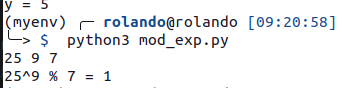
\includegraphics[width=10cm]{images/mod_exp_prueba.png}
        \caption{Ejecución de prueba del algoritmo de exponenciación modular}
    \end{figure}

\subsection{ALGORITMO DE DIVISIONES SUCESIVAS}
    \subsubsection{IMPLEMENTACIÓN}
\begin{lstlisting}[language=Python]
def divisiones_sucesivas(n):
    factores = []
    while n % 2 == 0:
        factores.append(2)
        n //= 2
    for i in range(3, int(n**0.5) + 1, 2):
        while n % i == 0:
            factores.append(i)
            n //= i
    if n > 2:
        factores.append(n)
    
    return factores
\end{lstlisting}

\subsubsection{EJEMPLO NÚMERICO}
Encontrar los factores primos de $1759875$, se prueba diviendo por todos los primos que sean $p_i$ tal que $p_i \leq \sqrt(n)$ y sean divisores de $n$.
\begin{align*} 
    1759875 / 3 & = 586625 \\
    586625 / 5 & = 117325 \\
    117325 / 5 & = 23465 \\
    23465 / 5 & =  4693\\
    4693 / 13 & =  361\\
    361 / 19 & =  19\\
    19 / 19 & =  1\\
    &\Rightarrow factores(1759875) = [3, 5^3, 13, 19^2]
\end{align*}

\subsubsection{EJEMPLO DE EJECUCIÓN}
\begin{figure}[H]
    \centering
    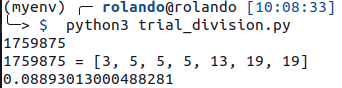
\includegraphics[width=10cm]{images/trial_divition_prueba.png}
    \caption{Ejecución de prueba del algoritmo de factorización por divisiones sucesivas}
\end{figure}


\subsection{MÉTODO DE DIFERENCIA DE CUADRADOS DE FERMAT}
\subsubsection{IMPLEMENTACIÓN}
\begin{lstlisting}[language=Python]
import math

def factorizacion_fermat(n):
    if n % 2 == 0:
        return (2, n // 2)

    a = math.ceil(math.sqrt(n))
    b2 = a * a - n

    while not es_cuadrado_perfecto(b2):
        a += 1
        b2 = a * a - n

    b = int(math.sqrt(b2))
    return (a - b, a + b)

def es_cuadrado_perfecto(x):
    s = int(math.isqrt(x))
    return s * s == x
\end{lstlisting}

\subsubsection{EJEMPLO NÚMERICO}
    Encontrar los factores primos de $5959$
    \begin{align*}
        a &= \lceil \sqrt{5959} \rceil \\
        a &= 78\\
        b^2 &= a^2 - n\\
        b^2 &= 78^2 - 5959\\
        b^2 &= 6084 - 5959\\
        b^2 &= 125
    \end{align*}
    Verificamos si $b^2$ es cuadrado perfecto:
    \begin{align*}
        \sqrt{125} & \approx 11.18 
    \end{align*}
    Como no es cuadrado perfecto se incrementa $a$ y se repite:
    \begin{align*}
        a &= 79\\
        b^2 &= 79^2 - 5959\\
        b^2 &= 282 \\
        \sqrt{282} &\approx 16.79 \\
        a &= 80\\
        b^2 &= 80^2 - 5959\\
        b^2 &= 441 \\
        \sqrt{441} &= 21 \\
    \end{align*}
    Como $441$ es cuadrado perfecto se han encontrado $a=80$ y $b=21$, y su factorización es:
    \begin{align*} 
        n &=  (a+b)(a-b)\\ 
        n &=  (80+21)(80-21)\\
        x &=  (101)(59)\\
    \end{align*}

    \subsubsection{EJEMPLO DE EJECUCIÓN}
    \begin{figure}[H]
        \centering
        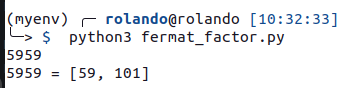
\includegraphics[width=10cm]{images/fermat_prueba.png}
        \caption{Ejecución de prueba del algoritmo de Fermat}
    \end{figure}

\subsection{ALGORITMO DE FACTORIZACIÓN EN UNA LINEA DE HART}
\subsubsection{IMPLEMENTACIÓN}
\begin{lstlisting}[language=Python]
import math

def factorizacion_hart(n, l):
    s = 1
    t = 1
    for i in range(1, l):
        s = math.ceil(math.sqrt(n*i))
        m = mod_exp(s, 2, n)
        t = math.isqrt(m)
        if t*t == m:
            break
    return gcd(s-t, n)
\end{lstlisting}
\subsubsection{EJEMPLO NÚMERICO}
    Factorizar $13290059$ con el algoritmo de factorización en una linea de Hart
    \begin{align*} 
        s &=  \lceil \sqrt{13290059\cdot 1}\rceil\\ 
        s &= 3646\\ 
        m &= 3646^2 \% 13290059\\ 
        m &= 3257\\
        \sqrt{m} &\approx  57.07\\
        \dots \\
        s &=  \lceil \sqrt{13290059\cdot 165}\rceil\\ 
        s &= 46828\\ 
        m &= 46828^2 \% 13290059\\
        m &= 1849\\
        t &=  \sqrt{m}\\
        t &=  \sqrt{1849}\\
        t &= 43\\
        gcd(s-t, n) &= gcd(46828-43, 13290059)\\
        &= 3119\\
    \end{align*}

    \subsubsection{EJEMPLO DE EJECUCIÓN}
    \begin{figure}[H]
        \centering
        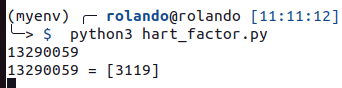
\includegraphics[width=10cm]{images/hart_prueba.png}
        \caption{Ejecución de prueba del algoritmo de factorización en una linea de Hart}
    \end{figure}


\subsection{MÉTODO DE POLLARD RHO}
\subsubsection{IMPLEMENTACIÓN}
\begin{lstlisting}[language=Python]
def pollard_rho(n):
    if n % 2 == 0:
        return 2

    x = random.randint(2, n - 1)
    y = x
    c = random.randint(1, n - 1)
    d = 1

    while d == 1:
        x = (mod_exp(x, 2, n) + c + n) % n
        y = (mod_exp(y, 2, n) + c + n) % n
        y = (mod_exp(y, 2, n) + c + n) % n
        d = gcd(abs(x - y), n)

    if d == n:
        return pollard_rho(n)

    return d
\end{lstlisting}

\subsubsection{EJEMPLO NÚMERICO}
    Factorizar $8051$ usando el algoritmo Pollard-Rho
    \begin{align*} 
        x &=  2\\
        y &=  2\\
        c &=  1\\ 
        d &= 1 \\
        x &= ((x^2)\%n + c + n)\%n\\
        x_0 &= (2^2\%8051 + 1 + 8051) \% 8051\\
        x_0 &= 5\\
        y_0 &= (2^2\%8051 + 1 + 8051) \% 8051\\
        y_0 &= 5\\
        y_1 &= (5^2\%8051 + 1 + 8051) \% 8051\\
        y_1 &= 26\\
        d &= gcd(|x-y|, n)\\
        d &= gcd(|5-26|, 8051)\\
        d &= 1
    \end{align*}

    \begin{align*} 
        x_1 &= (5^2\%8051 + 1 + 8051) \% 8051\\
        x_1 &= 26\\
        y_2 &= (26^2\%8051 + 1 + 8051) \% 8051\\
        y_2 &= 677\\
        y_3 &= (677^2\%8051 + 1 + 8051) \% 8051\\
        y_3 &= 7474\\
        d &= gcd(|26-7474|, 8051)\\
        d &= 1
    \end{align*}

    \begin{align*} 
        x_2 &= (26^2\%8051 + 1 + 8051) \% 8051\\
        x_2 &= 677\\
        y_2 &= (7474^2\%8051 + 1 + 8051) \% 8051\\
        y_2 &= 2839\\
        y_3 &= (2839^2\%8051 + 1 + 8051) \% 8051\\
        y_3 &= 871\\
        d &= gcd(|677-871|, 8051)\\
        d &= 97
    \end{align*}

    \subsubsection{EJEMPLO DE EJECUCIÓN}
    \begin{figure}[H]
        \centering
        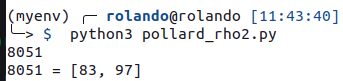
\includegraphics[width=10cm]{images/pollard_rho_prueba.png}
        \caption{Ejecución de prueba del algoritmo Pollard-Rho}
    \end{figure}

% \subsection{MÉTODO P-1 DE POLLARD}
% \subsubsection{IMPLEMENTACIÓN}
% \begin{lstlisting}[language=Python]
% import math
% from math import gcd
% from sympy import primerange

% def pollards_p_minus_1(n, B):
%     a = 2
    
%     M = 1
%     for p in primerange(2, B + 1)::
%         e = math.floor(math.log(n) / math.log(p))
%         M *= pow(p, e)
    
%     aM = mod_exp(a, M, n)
    
%     d = gcd(aM - 1, n)
    
%     if 1 < d < n:
%         return d
%     else:
%         return None
% \end{lstlisting}

% \subsubsection{EJEMPLO NÚMERICO}
%     Encontrar el resultado para $25^9 \% 7$
%     \begin{align*} 
%         x &=  25^9 \% 7\\ 
%         x &=  (25^4 \% 7)^2 (\times 25\cdot1) \% 7 \\
%         x &=  ((25^2 \% 7)^2)^2 \times (25 \% 7)\\
%         x &=  ((25\cdot25 \% 7)^2)^2 \times (25 \% 7)\\
%         x &=  (((625 \% 7)^2)^2 \times 4)\%7\\
%         x &=  (((2)^2)^2 \% 7 \times 4) mod 7\\
%         x &= ((4^2)\% 7 \times 4) \% 7\\
%         x &= (16 \% 7 \times 4) \% 7 \\
%         x &= (2 \times 4) \% 7 \\
%         x &= 8 \% 7 \\
%         x &= 1
%     \end{align*}

%     \subsubsection{EJEMPLO DE EJECUCIÓN}
%     \begin{figure}[H]
%         \centering
%         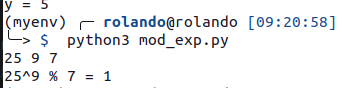
\includegraphics[width=10cm]{images/mod_exp_prueba.png}
%         \caption{Ejecución de prueba del algoritmo de exponenciación modular}
%     \end{figure}

\subsection{ALGORITMO DE FACTORIZACIÓN DE ENTEROS DE FRACCIONES CONTINUAS}
\subsubsection{IMPLEMENTACIÓN}
\begin{lstlisting}[language=Python]
import math

def fraccion_continua_sqrt(n):
    a0 = int(math.isqrt(n))
    if a0 * a0 == n:
        return [a0]
    
    cf = []
    m = 0
    d = 1
    a = a0
    cf.append(a)
    
    while a != 2 * a0:
        m = d * a - m
        d = (n - m * m) // d
        a = (a0 + m) // d
        cf.append(a)
    return cf

def convergentes(cf):
    h1, h2 = 1, 0
    k1, k2 = 0, 1
    convergentes_list = []
    
    for i in range(len(cf)):
        h = cf[i] * h1 + h2
        k = cf[i] * k1 + k2
        convergentes_list.append((h, k))
        h2, h1 = h1, h
        k2, k1 = k1, k
    return convergentes_list

def factorizar_fracciones_continuas(n):
    cf = fraccion_continua_sqrt(n)
    convs = convergentes(cf)
    
    for h, k in convs:
        if k == 0:
            continue
        x = h
        y = (x * x - n) // k
        
        if y >= 0 and int(math.isqrt(y)) ** 2 == y:
            factor = gcd(x + int(math.isqrt(y)), n)
            if 1 < factor < n:
                return factor
    
    return None
\end{lstlisting}

% \subsubsection{EJEMPLO NÚMERICO}
%     Encontrar el resultado para $25^9 \% 7$
%     \begin{align*} 
%         x &=  25^9 \% 7\\ 
%         x &=  (25^4 \% 7)^2 (\times 25\cdot1) \% 7 \\
%         x &=  ((25^2 \% 7)^2)^2 \times (25 \% 7)\\
%         x &=  ((25\cdot25 \% 7)^2)^2 \times (25 \% 7)\\
%         x &=  (((625 \% 7)^2)^2 \times 4)\%7\\
%         x &=  (((2)^2)^2 \% 7 \times 4) mod 7\\
%         x &= ((4^2)\% 7 \times 4) \% 7\\
%         x &= (16 \% 7 \times 4) \% 7 \\
%         x &= (2 \times 4) \% 7 \\
%         x &= 8 \% 7 \\
%         x &= 1
%     \end{align*}

    \subsubsection{EJEMPLO DE EJECUCIÓN}
    \begin{figure}[H]
        \centering
        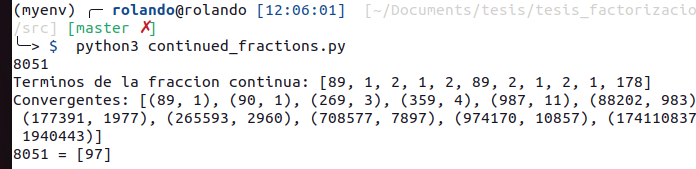
\includegraphics[width=10cm]{images/fracciones_continuas_pruebas.png}
        \caption{Ejecución de prueba del algoritmo de factorización con fracciones continuas}
    \end{figure}

\subsection{ALGORITMO DE FACTORIZACIÓN CON CURVAS ELÍPTICAS}
\subsubsection{IMPLEMENTACIÓN}
\begin{lstlisting}[language=Python]
def inverso_modular(a, p):
    g, x, _ = gcd_extendido(a, p)
    return x % p

def adicion_curva_eliptica(P, Q, a, p):
    if P == Q:
        lam = (3 * P[0] * P[0] + a) * inverso_modular(2 * P[1], p) % p
    else:
        lam = (Q[1] - P[1]) * inverso_modular(Q[0] - P[0], p) % p

    x3 = (lam * lam - P[0] - Q[0]) % p
    y3 = (lam * (P[0] - x3) - P[1]) % p

    return (x3, y3)

def multiplicacion_curva_eliptica(k, P, a, p):
    R = (0, 0)
    Q = P
    while k > 0:
        if k % 2 == 1:
            R = adicion_curva_eliptica(R, Q, a, p)
        Q = adicion_curva_eliptica(Q, Q, a, p)
        k //= 2
    return R

def ecm(n, B1=10000, B2=100000):
    while True:
        x = random.randint(1, n - 1)
        y = random.randint(1, n - 1)
        a = random.randint(1, n - 1)
        b = (y * y - x * x * x - a * x) % n

        if (4 * a * a * a + 27 * b * b) % n == 0:
            continue

        P = (x, y)
        for k in range(2, B1):
            P = multiplicacion_curva_eliptica(k, P, a, n)
            g = gcd(P[1], n)
            if 1 < g < n:
                return g


        for k in range(B1, B2):
            P = multiplicacion_curva_eliptica(k, P, a, n)
            g = gcd(P[1], n)
            if 1 < g < n:
                return g
\end{lstlisting}

% \subsubsection{EJEMPLO NÚMERICO}
%     Encontrar el resultado para $25^9 \% 7$
%     \begin{align*} 
%         x &=  25^9 \% 7\\ 
%         x &=  (25^4 \% 7)^2 (\times 25\cdot1) \% 7 \\
%         x &=  ((25^2 \% 7)^2)^2 \times (25 \% 7)\\
%         x &=  ((25\cdot25 \% 7)^2)^2 \times (25 \% 7)\\
%         x &=  (((625 \% 7)^2)^2 \times 4)\%7\\
%         x &=  (((2)^2)^2 \% 7 \times 4) mod 7\\
%         x &= ((4^2)\% 7 \times 4) \% 7\\
%         x &= (16 \% 7 \times 4) \% 7 \\
%         x &= (2 \times 4) \% 7 \\
%         x &= 8 \% 7 \\
%         x &= 1
%     \end{align*}

    \subsubsection{EJEMPLO DE EJECUCIÓN}
    \begin{figure}[H]
        \centering
        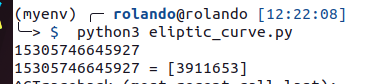
\includegraphics[width=10cm]{images/curva_eliptica_prueba.png}
        \caption{Ejecución de prueba del algoritmo de factorización con curvas Elipticas (ECM)}
    \end{figure}

\subsection{CRIBA DE ERATOSTENES}
\subsubsection{IMPLEMENTACIÓN}
\begin{lstlisting}[language=Python]
def sieve_of_eratosthenes(n):
    primes = [True] * (n + 1)
    p = 2
    while p * p <= n:
        if primes[p]:
            for i in range(p * p, n + 1, p):
                primes[i] = False
        p += 1
    return [p for p in range(2, n + 1) if primes[p]]
\end{lstlisting}
\subsubsection{EJEMPLO NÚMERICO}
    En la Figura \ref{eratostenes} se puede ver el resultado despues de ejecutar la criba de Eratostenes hasta 120, y a la derecha los primos encontrados
    \begin{figure}[H]
        \centering
        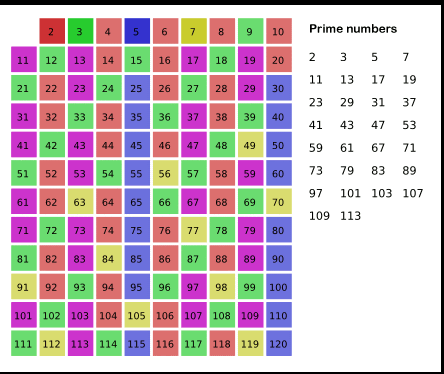
\includegraphics[width=10cm]{images/eratostenes_ejemplo.png}
        \caption{Resultado de la criba de Eratostenes}
        \label{eratostenes}
    \end{figure}

    % \subsubsection{EJEMPLO DE EJECUCIÓN}
    % \begin{figure}[H]
    %     \centering
    %     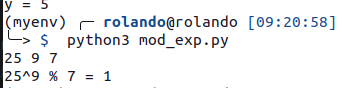
\includegraphics[width=10cm]{images/mod_exp_prueba.png}
    %     \caption{Ejecución de prueba del algoritmo de exponenciación modular}
    % \end{figure}

% \subsection{CRIBA MODIFICADA DE ERATOSTENES}
% \subsubsection{IMPLEMENTACIÓN}
% \begin{lstlisting}[language=Python]
% def sieve_interval_excluding_factors(I, J, P):
%     interval_size = J - I + 1
%     sieve = [True] * interval_size

%     for prime in P:
%         start = max(prime * prime, I + (prime - I % prime) % prime)
%         for multiple in range(start, J + 1, prime):
%             sieve[multiple - I] = False

    
%     result = [num for num, is_prime in zip(range(I, J + 1), sieve) if is_prime]
%     return result
% \end{lstlisting}

% \subsubsection{EJEMPLO NÚMERICO}
%     Encontrar el resultado para $25^9 \% 7$
%     \begin{align*} 
%         x &=  25^9 \% 7\\ 
%         x &=  (25^4 \% 7)^2 (\times 25\cdot1) \% 7 \\
%         x &=  ((25^2 \% 7)^2)^2 \times (25 \% 7)\\
%         x &=  ((25\cdot25 \% 7)^2)^2 \times (25 \% 7)\\
%         x &=  (((625 \% 7)^2)^2 \times 4)\%7\\
%         x &=  (((2)^2)^2 \% 7 \times 4) mod 7\\
%         x &= ((4^2)\% 7 \times 4) \% 7\\
%         x &= (16 \% 7 \times 4) \% 7 \\
%         x &= (2 \times 4) \% 7 \\
%         x &= 8 \% 7 \\
%         x &= 1
%     \end{align*}

%     \subsubsection{EJEMPLO DE EJECUCIÓN}
%     \begin{figure}[H]
%         \centering
%         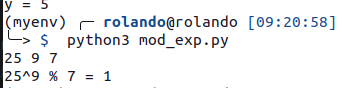
\includegraphics[width=10cm]{images/mod_exp_prueba.png}
%         \caption{Ejecución de prueba del algoritmo de exponenciación modular}
%     \end{figure}

\subsection{CRIBA CUADRATICA}
\subsubsection{IMPLEMENTACIÓN}
\begin{lstlisting}[language=Python]
def quad_residue(a,n):
    l=1
    q=(n-1)//2
    x = q**l
    if x==0:
        return 1
        
    a =a%n
    z=1
    while x!= 0:
        if x%2==0:
            a=(a **2) % n
            x//= 2
        else:
            x-=1
            z=(z*a) % n
    return z

def STonelli(n, p):
    q = p - 1
    s = 0
    while q % 2 == 0:
        q //= 2
        s += 1
    if s == 1:
        r = pow(n, (p + 1) // 4, p)
        return r,p-r
    for z in range(2, p):
        if p - 1 == quad_residue(z, p):
            break
    c = pow(z, q, p)
    r = pow(n, (q + 1) // 2, p)
    t = pow(n, q, p)
    m = s
    t2 = 0
    while (t - 1) % p != 0:
        t2 = (t * t) % p
        for i in range(1, m):
            if (t2 - 1) % p == 0:
                break
            t2 = (t2 * t2) % p
        b = pow(c, 1 << (m - i - 1), p)
        r = (r * b) % p
        c = (b * b) % p
        t = (t * c) % p
        m = i
    return (r,p-r)

def is_probable_prime(a):
    if a == 2:
        return True

    if a == 1 or a % 2 == 0:
        return False

    return rabin_miller_primality_test(a, 50)

def rabin_miller_primality_test(a, iterations):
    r, s = 0, a - 1

    while s % 2 == 0:
        r += 1
        s //= 2

    for _ in range(iterations):
        n = randint(2, a - 1)
        x = pow(n, s, a)
        if x == 1 or x == a - 1:
            continue
        for _ in range(r - 1):
            x = pow(x, 2, a)
            if x == a - 1:
                break
        else:
            return False
    return True

def prime_gen(n):
    if n < 2:
        return []
    
    nums = []
    isPrime = []
    
    for i in range(0, n+1):
        nums.append(i)
        isPrime.append(True)
        
    isPrime[0]=False
    isPrime[1]=False
    
    for j in range(2,int(n/2)):
        if isPrime[j] == True:
            for i in range(2*j,n+1,j):
                isPrime[i] = False
                
    primes = []
    for i in range(0, n+1):
        if isPrime[i] == True:
            primes.append(nums[i])
            
    return primes

def isqrt(n):
    x = n
    y = (x + 1) // 2
    while y < x:
        x = y
        y = (x + n // x) // 2
    return x

def find_base(N,B):
    factor_base = []
    primes = prime_gen(B)
    for p in primes:
        if quad_residue(N,p) == 1:
            factor_base.append(p)
    return factor_base

def find_smooth(factor_base,N,I):
    def sieve_prep(N,sieve_int):
        sieve_seq = [x**2 - N for x in range(root,root+sieve_int)]
        return sieve_seq

    sieve_seq = sieve_prep(N,I)
    sieve_list = sieve_seq.copy()
    if factor_base[0] == 2:
        i = 0
        while sieve_list[i] % 2 != 0:
            i += 1
        for j in range(i,len(sieve_list),2):
            while sieve_list[j] % 2 == 0:
                sieve_list[j] //= 2
    for p in factor_base[1:]:
        residues = STonelli(N,p)
        for r in residues:
            for i in range((r-root) % p, len(sieve_list), p):
                while sieve_list[i] % p == 0:
                    sieve_list[i] //= p
    xlist = []
    smooth_nums = []
    indices = []
    
    for i in range(len(sieve_list)):
        if len(smooth_nums) >= len(factor_base)+T:
            break
        if sieve_list[i] == 1:
            smooth_nums.append(sieve_seq[i])
            xlist.append(i+root)
            indices.append(i)
    return(smooth_nums,xlist,indices)

def build_matrix(smooth_nums,factor_base):
    def factor(n,factor_base):
        factors = []
        if n < 0:
            factors.append(-1)
        for p in factor_base:
            if p == -1:
                pass
            else:
                while n % p == 0:
                    factors.append(p)
                    n //= p
        return factors

    M = []
    factor_base.insert(0,-1)
    for n in smooth_nums:
        exp_vector = [0]*(len(factor_base))
        n_factors = factor(n,factor_base)
        for i in range(len(factor_base)):
            if factor_base[i] in n_factors:
                exp_vector[i] = (exp_vector[i] + n_factors.count(factor_base[i])) % 2
        if 1 not in exp_vector:
            return True, n
        else:
            pass
        
        M.append(exp_vector)
    return(False, transpose(M))

def transpose(matrix):
    new_matrix = []
    for i in range(len(matrix[0])):
        new_row = []
        for row in matrix:
            new_row.append(row[i])
        new_matrix.append(new_row)
    return(new_matrix)

def solve(solution_vec,smooth_nums,xlist,N):
    solution_nums = [smooth_nums[i] for i in solution_vec]
    x_nums = [xlist[i] for i in solution_vec]
    Asquare = 1
    for n in solution_nums:
        Asquare *= n
    b = 1
    for n in x_nums:
        b *= n
    a = isqrt(Asquare)
    factor = gcd(b-a,N)
    return factor

def solve_row(sol_rows,M,marks,K=0):
    solution_vec, indices = [],[]
    free_row = sol_rows[K][0]
    for i in range(len(free_row)):
        if free_row[i] == 1: 
            indices.append(i)
    for r in range(len(M)):
        for i in indices:
            if M[r][i] == 1 and marks[r]:
                solution_vec.append(r)
                break
            
    solution_vec.append(sol_rows[K][1])       
    return(solution_vec)

def gauss_elim(M):
    marks = [False]*len(M[0])
    
    for i in range(len(M)):
        row = M[i]
        for num in row:
            if num == 1:
                j = row.index(num)
                marks[j] = True
                
                for k in chain(range(0,i),range(i+1,len(M))):
                    if M[k][j] == 1:
                        for i in range(len(M[k])):
                            M[k][i] = (M[k][i] + row[i])%2
                break
    M = transpose(M)
    sol_rows = []
    for i in range(len(marks)):
        if marks[i]== False:
            free_row = [M[i],i]
            sol_rows.append(free_row)
    return sol_rows,marks,M

def QS(n,B,I):    
    global N
    global root
    global T
    N,root,K,T = n,int(sqrt(n)),0,1
    
    if isinstance(sqrt(N),int):
        return isqrt(N)
    factor_base = find_base(N,B)
    global F
    F = len(factor_base)
    smooth_nums,xlist,indices = find_smooth(factor_base, N,I)
    is_square, t_matrix = build_matrix(smooth_nums,factor_base)
    
    if is_square == True:
        x = smooth_nums.index(t_matrix)
        factor = gcd(xlist[x]+sqrt(t_matrix),N)
        return factor, N/factor
    sol_rows,marks,M = gauss_elim(t_matrix)
    solution_vec = solve_row(sol_rows,M,marks,0)
    factor = solve(solution_vec,smooth_nums,xlist,N)

    for K in range(1,len(sol_rows)):
        if (factor == 1 or factor == N):
            solution_vec = solve_row(sol_rows,M,marks,K)
            factor = solve(solution_vec,smooth_nums,xlist,N)
        else:
            return factor, int(N/factor)
\end{lstlisting}

\subsubsection{EJEMPLO DE EJECUCIÓN}
\begin{figure}[H]
    \centering
    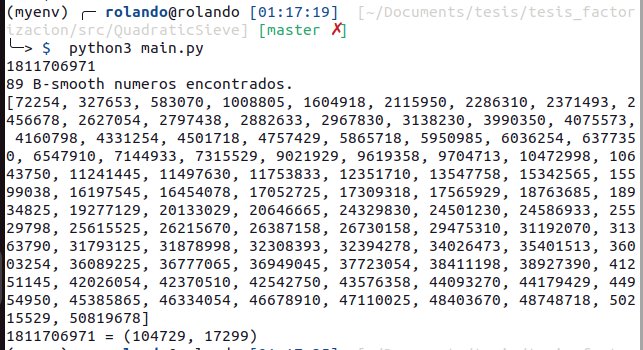
\includegraphics[width=10cm]{images/criba_cuadratica_prueba.png}
    \caption{Resultado de la criba de Cuadratica}
    \label{eratostenes}
\end{figure}